\documentclass[10pt]{beamer}

\usepackage[UTF8,noindent]{ctex}
\usepackage{times}
\usepackage{fontenc}
\usetheme{Boadilla}
\setbeamertemplate{navigation symbols}{}
\setbeamertemplate{background}{
\includegraphics[height=\paperheight]{bg}}
\title[中期答辩]{“卷皮网”用户画像及精准推荐实战}
\subtitle{大学生创新训练项目中期答辩}
\author[用户画像与机器学习实战]{答辩人:孙嘉轩\ 黄爽\ 龙海文\ 杨岳浩\ 许艳\newline \newline 指导老师:张千帆}
\institute[]{华中科技大学管理学院}

%%%%%%%%%%%%%%%%%%%%%%%%%%%%%%%%%%
\begin{document}
%%%%%%%%%%%%%%%%%%%%%%%%%%%%%%%%%%

\frame{\titlepage}
\begin{frame}
\textbf{"There is nothing about doing data analysis that is neutral.\newline
What and how data is collected, how the data is cleaned\newline and
stored, what models are constructed, and what questions are
asked – all of this is political."}
\newline Danah Boyd, NYU

\end{frame}

\begin{frame}{目录}
\tableofcontents
\end{frame}

\section{项目进展}

\begin{frame}{专业知识与技能}
\begin{itemize}
\item 机器学习与数据挖掘基本概念与使用方法\newline
\item 从商业分析角度探究用户画像在企业中的应用\newline
\item 使用R/Python等编程语言进行分析与研究\newline
\end{itemize}
\end{frame}

\begin{frame}{企业合作}
  \begin{itemize}
  \item 与卷皮网员工进行交流
  \newline
  \item 爬取并分析卷皮网相关数据
  \newline
  \item 发现数据潜在商业价值与市场应用
  \end{itemize}
\end{frame}

\begin{frame}{方案优化}
  \textbf{项目执行中的问题}\newline
   \begin{itemize}
      \item 卷皮网购物数据质量较低,用户类型单一,不具有普遍意义。\newline
      \item 一个项目无法全面展现机器学习中丰富的研究方法。\newline
      \item 不同应用场景下的用户画像有很大区别。\newline
      \item 报告的形式无法很好的呈现研究结果。
   \end{itemize}
\end{frame}

\begin{frame}{方案优化}
  \textbf{解决方案与改进措施}\newline
   \begin{itemize}
      \item 增加研究领域,扩大研究范围,全方位解读用户画像的企业应用场景。\newline
      \item 增加对于不同数据类型、不同方法的对比研究。对比不同编程语言及程序包的优劣。\newline
      \item 通过建立网页版教程,系统归纳团队研究过程及心得,给入门用户提供学习的平台。\newline
      \item 编写入门级机器学习实践案例,增强教程的实践性与互动性。
   \end{itemize}
\end{frame}


\begin{frame}{网页}
\begin{columns}
  \begin{column}{0.4\textwidth}
    \textbf{userprofileguide.github.io}
  \end{column}
  \begin{column}{0.6\textwidth}
    
\includegraphics[height=0.4\paperheight]{website1}
    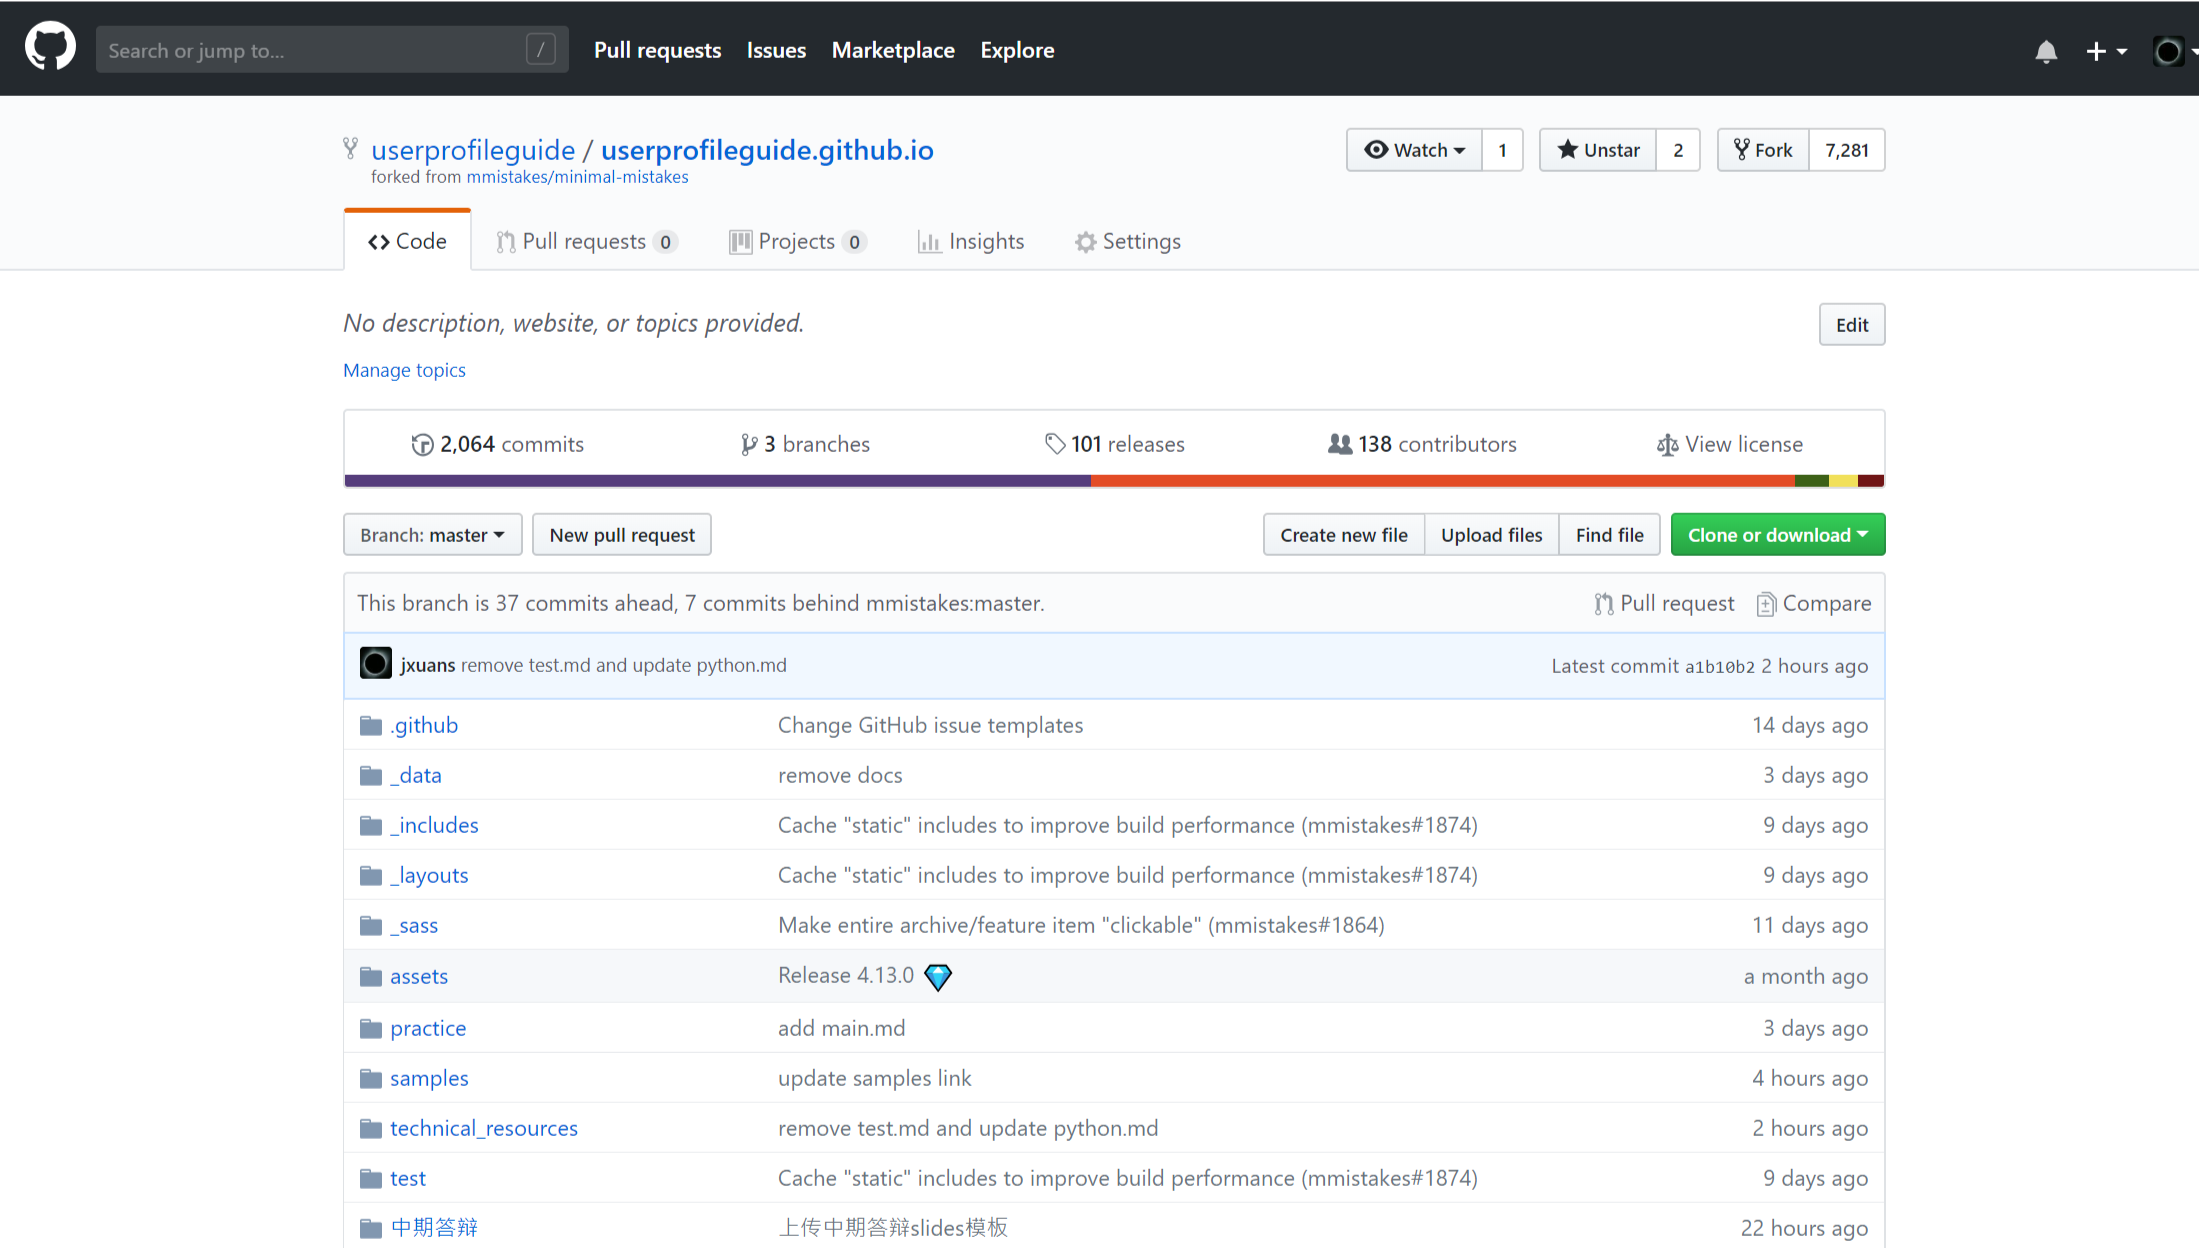
\includegraphics[height=0.4\paperheight]{website2}
  \end{column}
  \end{columns}
\end{frame}

\begin{frame}{网页}
\textbf{教程框架设计}
\begin{itemize}
\item 技术原理:对概念和基础知识点的介绍、程序包的使用方法介绍、算法原理介绍等。\newline
\item 案例分析:全面记录团队项目开发过程和在其中使用到的研究方法、编程技巧、优化思路,并进行探讨比较。\newline
\item 入门练习:提供让入门读者快速上手实践并理解机器学习和用户画像的案例,数据与源代码。\newline
\end{itemize}
\end{frame}
%%%%%%

\section{现阶段问题}
  \begin{frame}{现阶段问题}
    \begin{itemize}
      \item 企业数据获得较为困难,企业严格限制API的调用。\newline
      \item 已有中文语义分析技术尚不成熟,对中文用户刻画精确度较低。\newline
      \item 尚未明确针对不同行业设计数据清理方案的思路。
    \end{itemize}
  \end{frame}

%%%%%%

\section{财务情况}
  \begin{frame}{}
  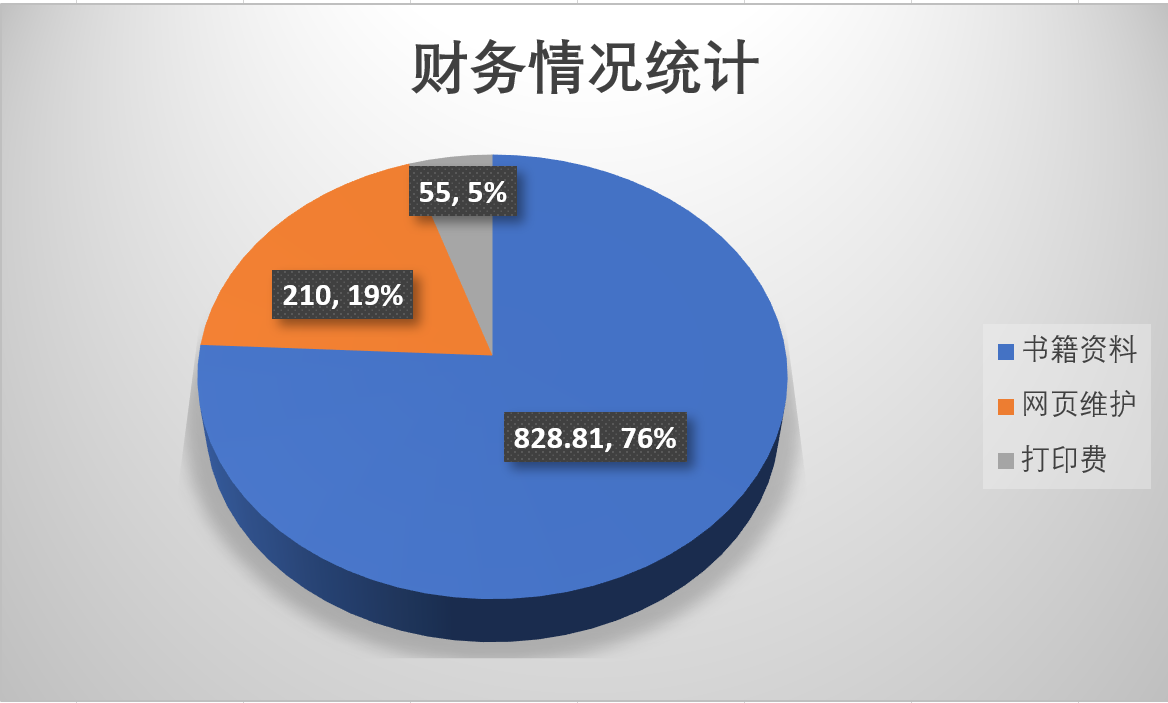
\includegraphics[height=0.66\paperheight]{finance}
  \end{frame}

%%%%%%

\section{后续工作安排}
\begin{frame}{后续工作安排}
  \begin{itemize}
    \item 拓宽研究领域,完成更多项目开发案例。\newline
    \item 继续完善教程主体部分和延申部分,增强内容的完整度与可读性。\newline
    \item 与企业进行合作,进一步探讨用户画像的商业价值与伦理学边界。\newline
    \item 扩大影响力,打造可持续发展编程社区,不断引入更多优质内容,吸引越来越多的同行加入。
  \end{itemize}

\end{frame}


%%%%%%

\begin{frame}
\textbf{感谢聆听!}
\end{frame}


\end{document}
